%\RequirePackage{fixltx2e}
\RequirePackage{fix-cm}

\documentclass[%
10pt,
pdf,
intlimits,
sumlimits,
namelimits,
fleqn,
russian,
noamsthm,
hyperref={unicode},
% Использование шрифтов с засечками
% mathserif,
% serif,
utf8,
% ignorenonframetext,
usepdftitle={false}, % не вставлять информацию из переменных \author \title
% aspectratio=16:9
\ifdefined\aspectXVIxIX
aspectratio=169,
\else\fi
\ifdefined\printable
%8pt,
%a4paper,
handout,
\else\fi
]{beamer}

% Нумерованые подписи к рисункам и таблицам
\setbeamertemplate{caption}[numbered]

\setbeamerfont{caption}{size=\footnotesize}
\setbeamertemplate{caption label separator}{.}

% Нумерация литературы, если нужно использовать \cite
% по-умолчанию литература обозначается иконками
\setbeamertemplate{bibliography item}[text]

% Поддержка русского языка
\uselanguage{Russian}

% Поддержка приложений
\usepackage{appendixnumberbeamer}

\usepackage[utf8]{inputenc} % распознование кодировки текста в tex-файле
\usepackage[T2A]{fontenc} % распознование шрифтов

\renewcommand{\familydefault}{\sfdefault}
\renewcommand\mathfamilydefault{\rmdefault}%

\usepackage[english, main=russian]{babel}% пакет поддержки орфографий


\usepackage{etex}

% расширенное управление переносом слов, разделенных пунктиром
\usepackage[shortcuts]{extdash}
% поддержка настроек междустрочного интервала
\usepackage{setspace}
% Настройка сносок
\usepackage[perpage,bottom,multiple,stable]{footmisc}

%% Пакеты для гипертекста
\RequirePackage{color} %
\usepackage{hyperref} % обширная поддержка гипертекста
\hypersetup{backref,
% colorlinks=false,
linktoc=all
}
\hypersetup{pdfborder=0 0 0}
\hypersetup{pdfencoding=auto}

%% Расширенная математика
\usepackage{amsmath}
\usepackage{amssymb}
\usepackage{amsthm}
\usepackage{amscd}

\usepackage{accents} % пользовательские акценты
\usepackage{cmap} % предоставляет таблицы сопоставления символов для PDF
\usepackage{textcomp} % поддержка шрифтов Text Companion
\usepackage{mathtext} % для "прозрачного" использования кириллических букв в формулах

\usepackage{mathtools}
\mathtoolsset{
showonlyrefs=true, % нумеровать только формулы, на которых есть ссылки
mathic=true,
}

\allowdisplaybreaks

% Поддержка перечислений и списков
%\usepackage{enumerate} % классической пакет
\usepackage{paralist}
%\usepackage{enumitem} % не совместим с пакетом paralist
% см. о разнице кратко https://tex.stackexchange.com/questions/18411/what-are-the-differences-between-using-paralist-vs-enumitem

%% Многостраничные таблицы
% \usepackage{longtable}
% \usepackage{lscape}
% \usepackage{makecell}
% \usepackage{multirow}
% \usepackage{tabularx}
% или
\usepackage{tabularray}
\UseTblrLibrary{functional}
\UseTblrLibrary{diagbox}

\DefTblrTemplate{contfoot-text}{russian}{Продолжение на следующей странице}
\SetTblrTemplate{contfoot-text}{russian}
\DefTblrTemplate{conthead-text}{russian}{(Продолжение)}
\SetTblrTemplate{conthead-text}{russian}


%% Работа с графикой
\usepackage{graphicx}

\usepackage{float}
\usepackage{epic}
\usepackage{rotating}
\usepackage[scanall]{psfrag}

\usepackage[shell, subfolder]{gnuplottex}
\def\gnuplotexe{/usr/bin/gnuplot}
% \def\gnuplotexe{C:/Program\ Files/gnuplot/bin/gnuplot.exe}

%% Путь к рисункам
\graphicspath{{images/}{gnuplottex/}}

%% Обработка текста в eps-файлах
\usepackage[scanall]{psfrag}

%% обработка блок-схем
\usepackage{tikz}
\usetikzlibrary{arrows, shapes, graphs, automata, positioning}

%% Пакеты для библиографии
\usepackage{cite}%
% \usepackage{gost7184}
% \bibliographystyle{gost7184}
% \bibliographystyle{ugost2003s}
\bibliographystyle{gost2008ls}
% \bibliographystyle{utf8gost780u}
%\renewcommand{\bibname}{Литература} % если класс book или report
\renewcommand{\refname}{Литература} % если класс article

%% Пакеты для листингов
%% Расширеное окружение verbatim
\usepackage{fancyvrb}

%{{{ Dirty hack

\makeatletter % fix the ligature list and hope for the best
\def\verbatim@nolig@list{\do\`\do\,\do\'\do\-}
\makeatother

%}}}

\usepackage{url}

% Наряду, или вместо verbatim можно использовать более специализированный.
% Пакет listings
\usepackage{listings}
\usepackage{listingsutf8}
\lstset{%
	showstringspaces=false,
	numbers=left,
	% numberstyle=\tiny,
	% upquote=false,
	keepspaces=true,
	columns=flexible,
	basicstyle=\footnotesize,%
	breaklines=true,%
	breakatwhitespace=true,%
	postbreak=\space,%
	prebreak={\mbox{\quad$\hookleftarrow$}},%
	title=\lstname ,%
	escapeinside={\%*}{*)}, %
	extendedchars=\true, %
% 	inputencoding=utf8,
% 	fontencoding=T2A,
}

%\ifthenelse{\boolean{luatex}\OR\boolean{xetex}}{}{%
%    \lstset{inputencoding=utf8/koi8-r}}

\lstloadlanguages{C,make,bash,[x86masm]Assembler,[LaTeX]TeX, [08]Fortran, [95]Fortran, Gnuplot}

\usepackage{indentfirst} % отступ первой строки каждого раздела по умолчанию
% \renewcommand\baselinestretch{1} % междустроный интервал всего документа

%\usepackage[newcommands, document]{ragged2e}

%~~~~~~~~~~~~~~~~~~~~~~~~~~~~~~~~~~~~~~~~~~~~~~~~~~~~~~~~~~~~~~~~~~~~~~~~~~~~~~~~~~~~~~~~~~~~~
%                                Тема оформления
%~~~~~~~~~~~~~~~~~~~~~~~~~~~~~~~~~~~~~~~~~~~~~~~~~~~~~~~~~~~~~~~~~~~~~~~~~~~~~~~~~~~~~~~~~~~~~
\usetheme{default}
% Возможные темы
% CambridgeUS, default, Bergen, Madrid, AnnArbor, Pittsburgh, Rochester,
% Antibes, Montpellier, Berkeley, Berlin, Frankfurt, PaloAlto, Ilmenau, Copenhagen,
% Warsaw

% Цветовая тема
\usecolortheme{dove}%1
\usecolortheme{crane}%2
\usecolortheme{orchid}%3
\usecolortheme{beaver}%4


% infolines tree
\useoutertheme{infolines}%1
\useoutertheme{tree}%2
% circles inmargin rectangles rounded
\useinnertheme[shadow]{rounded}%1
\useinnertheme{circles}%2

% serif structurebold structureitalicserif structuresmallcapsserif
\usefonttheme{professionalfonts}

% Убираем навигационные символы
% \setbeamertemplate{navigation symbols}{}

% Версия для печати
\ifdefined\printable
  \usecolortheme{dove}
  \setbeamertemplate{navigation symbols}{}
\fi


% \setbeamertemplate{section in toc}[default]
% \AtBeginSection[] {
% \begin{frame}
% \frametitle{Outline}
% \frametitle{Содержание}
% \tableofcontents[currentsection]
% \note{\tableofcontents[currentsection]}
% \end{frame}}

%~~~~~~~~~~~~~~~~~~~~~~~~~~~~~~~~~~~~~~~~~~~~~~~~~~~~~~~~~~~~~~~~~~~~~~~~~~~~~~~~~~~~~~~~~~~~~

\makeatletter
    \newenvironment{withoutheadline}{
        \setbeamertemplate{headline}[default]
        \def\beamer@entrycode{\vspace*{-\headheight}}
    }{}
    \newenvironment{withoutfootline}{
        \setbeamertemplate{footline}[default]
        \def\beamer@entrycode{\vspace*{+\footheight}}
    }{}
    \newenvironment{withoutheadandfootlines}{
        \setbeamertemplate{headline}[default]
        \def\beamer@entrycode{\vspace*{-\headheight}}
        \setbeamertemplate{footline}[default]
        \def\beamer@entrycode{\vspace*{+\footheight}}
    }{}
\makeatother

\ifx\pstmode\undefined
\else
    \setbeamertemplate{navigation symbols}{}
\fi

\ifdefined\withnotes
	\usepackage{pgfpages}

	\ifdefined\onlynotes
	\setbeameroption{show only notes}
	\setbeamertemplate{note page}[compress]
	\pgfpagesuselayout{resize to}[a4paper,border shrink=5mm,landscape]
	\else
	\setbeameroption{show notes}
	\setbeamertemplate{note page}[plain]
	\pgfpagesuselayout{8 on 1}[a4paper,border shrink=5mm]
	\fi

	% Версия для печати
	\ifdefined\printable
	  \usecolortheme{dove}
	  \setbeamertemplate{navigation symbols}{}
	  \setbeamercolor{note page}{bg=white}
	  \setbeamercolor{note title}{bg=white}
	  \setbeamercolor{note date}{bg=white}
	\fi

	% http://tex.stackexchange.com/questions/288408/beamer-show-notes-on-second-screen-with-xelatex-and-atbeginsection
	\ifthenelse{\boolean{xetex}}{%
	  \makeatletter
	  \def\beamer@framenotesbegin{% at beginning of slide
		 \usebeamercolor[fg]{normal text}
		 \gdef\beamer@noteitems{}%
		 \gdef\beamer@notes{}%
	  }
	  \makeatother
	}{}
\else\fi

\ifdefined\handoutwithnotes
	\usepackage{handoutWithNotes}
	\pgfpagesuselayout{4 on 1 with notes}[a4paper,border shrink=5mm]
\else\fi

\ifdefined\poster
	\mode<presentation> {
		 \usetheme{PFU}				% Название темы оформления для постера
		 \setbeamertemplate{navigation symbols}{}	% Убираем навигационные символы
	}

	\usepackage{ragged2e}
	\boldmath			% Математические формулы будут полужирными, чтоб в глаза било

	%\usepackage[orientation=album,size=a0,scale=1.4,debug]{beamerposter}                       	% e.g. for DIN-A0 poster
	%\usepackage[orientation=portrait,size=a1,scale=1.4,grid,debug]{beamerposter}                  	% e.g. for DIN-A1 poster, with optional grid and debug output
	%\usepackage[size=custom,width=200,height=120,scale=2,debug]{beamerposter}                     	% e.g. for custom size poster
	%\usepackage[orientation=portrait,size=a0,scale=1.0,printer=rwth-glossy-uv.df]{beamerposter}   	% e.g. for DIN-A0 poster with rwth-glossy-uv printer check
	%\usepackage[orientation=album,size=a0,scale=1.4]{beamerposter}
	\usepackage[orientation=portrait,size=a1,scale=1.0]{beamerposter}
\else\fi

\usepackage{pifont}

%% настройки геометрии
%\RequirePackage{xkeyval}

\usepackage{bm} % определяет команду \bm{<текст>} дающее полужирное начертание тексту <текст> в аргументе

\usepackage{texnames}

\usepackage{wrapfig} % позволяет обернуть текст вокруг рисунков или таблиц

\def\bibnamefont{\textit} % задаёт курсив Ф.И.О. авторов в списке литературы

\usepackage{calc}
\usepackage{soulutf8} % пакет soul с поддержкой utf8: позволяет быстро форматировать текст, например выделить командой \hl


% \usepackage[nodayofweek]{datetime}
\usepackage[24hr]{datetime}

\nocite{*} %  включает в спиcок литературы все записи что без ссылок в тектсе через \cite

\usepackage{afterpage}
\usepackage{subfigure}
\renewcommand{\thesubfigure}{\asbuk{subfigure}}

\begin{document}

\lstset{language = {[LaTeX]TeX}, frame = none, tabsize = 3, numbers = left, numbersep = 6pt, gobble=1}%, literate={\$}{{\textcolor{blue}{\$}}}1, literate={\%}{{\textcolor{blue}{\%}}}1}

\tikzset{terminator/.style = {% терминатор - начало или конец любой функции/подпрограммы
				rectangle, draw, text centered, rounded corners, minimum height = 2em
			}
		}
\tikzset{operator/.style = {% блок выполнения операций над данными
		rectangle, draw, text centered, minimum height = 2em
	}
}
\tikzset{decision/.style = {% блок оператора ветвления
		diamond, draw, text centered, minimum height = 2em
	}
}
\tikzset{data/.style = {% блок ввода-ввывода данных
		trapezium, draw, text centered, trapezium left angle = 60,
		trapezium right angle = 120, minimum height = 2em
	}
}
\tikzset{link/.style = {% связь
		draw, -latex'
	}
}
\tikzset{connector/.style = {% соединитель, есть штатный стиль "state"
		circle, draw, text centered, minimum height = 2em
	}
}
\tikzset{function/.style = {% блок вызова внешней функции
		rectangle split, rectangle split horizontal,
		rectangle split parts = 3,
		draw, text centered,
		minimum width = 5em,
		minimum height = 2em,
		outer sep = 0
	}
}
\tikzset{subroutine/.style = {% блок вызова внешней подпрограммы
		rectangle split, rectangle split horizontal,
		rectangle split parts = 3,
		draw, text centered,
		minimum width = 5em,
		minimum height = 2em,
		outer sep = 0
	}
}
\tikzset{procedure/.style = {% блок вызова внешней процедуры
		rectangle split, rectangle split horizontal,
		rectangle split parts = 3,
		draw, text centered,
		minimum width = 5em,
		minimum height = 2em,
		outer sep = 0
	}
}
\tikzset{loop/.style = {% блок-начало цикла с условием
		chamfered rectangle,
		chamfered rectangle corners={
			north west, north east
		},
		draw, text centered,
		minimum width = 5em,
		minimum height = 2em,
		outer sep = 0
	}
}
\tikzset{endloop/.style = {% блок-конец цикла с условием
		chamfered rectangle,
		chamfered rectangle corners={
			south west, south east
		},
		draw, text centered,
		minimum width = 5em,
		minimum height = 2em,
		outer sep = 0
	}
}
\tikzset{counterloop/.style = {% блок цикла со счётчиком
		chamfered rectangle,
		chamfered rectangle xsep = 2cm,
		draw, text centered,
		minimum width = 5em,
		minimum height = 2em,
		outer sep = 0
	}
}
\tikzset{preparation/.style = {% блок подготовки данных
		rectangle split, rectangle split horizontal,
		rectangle split parts = 3,
		draw, text centered,
		minimum width = 5em,
		minimum height = 2em,
		outer sep = 0
	}
}

%% титульная часть

\title[ЛиГ]{%
   {%\Large%
      Краткое введение в \LaTeX \\
		и основы работы с Gnuplot
   }
}

\subtitle[П]{%
   {\bfseries в примерах}
}

\author[Николаев~Н.~Э. и~др.]{Николаев~Н.~Э.\inst{1,2)}, Гоним~Н.\inst{1,3)}}

\institute[РУДН]{%
   \small \inst{1)} Институт физических исследований и технологий \\
   Российский университет дружбы народов \\
   Россия, 117198, Москва, ул. Миклухо-Маклая, 6 \\[1ex]
   \inst{2)}\lstinline|<nikolaev_ne@pfur.ru>|, \inst{3)}\lstinline|<gonim_m@pfur.ru>|
}

\subject{\LaTeX}

\date[ИФИТ]{%
   {\normalsize Лекция} \\[2ex]
   % {\small Научный семинар} \\
   %{\small Институт физических исследований и технологий} \\[1ex]
   {\footnotesize\bf Май} \\
   {\footnotesize\bf 2022}
}

\begin{withoutheadandfootlines}
   \begin{frame}[squeeze]
		\vspace*{-5ex}
      \maketitle
   \end{frame}
\end{withoutheadandfootlines}

%% Аннотация

\begin{frame}[squeeze]
	\label{frame:annotation}
	% \frametitle{Аннотация}
	\vspace\headheight
	\vspace*{-0.5ex}
	{\centering\bfseries%
		\large\underline{Аннотация} \\
	}
	\medskip

	\footnotesize\quad Рассматриваются некоторые возможности языка программирования \LaTeX\ для подготовки отчётов, научных статей и др. Приводятся примеры с небольшим пояснением, в том числе работа с математическими формулами, графиками, таблицами, листингом и блок\nobreak-схемами.
	\medskip

	\footnotesize\qquad{\bfseries Ключевые слова:} издательская система, язык программирования, построение графиков, построение таблиц, построение блок\nobreak-схем, \LaTeX, листинг, оформление математических выражений.
\end{frame}

%% Оглавление

\begin{withoutheadline}
   \begin{frame}[squeeze, fragile]%, allowframebreaks]
      \label{frame:contents}
      \frametitle{\contentsname}
      \vbox{%
         \usebeamerfont{frametitle}%
         \usebeamercolor{frametitle}%
         \color{fg}
         \vspace{2em}
         % \hbox{\usebeamerfont{frametitle}\insertframetitle}
         % \hbox{\usebeamerfont{framesubtitle}\insertframesubtitle}
      }
		\vspace*{-10em}
      \begin{minipage}[t][0.5cm]{\textwidth}
         {\footnotesize
            \tableofcontents
         }
      \end{minipage}
      \vfill
   \end{frame}
\end{withoutheadline}



% введение
\section{Введение}
\label{sec:introduction}


\begin{frame}[squeeze]
%    \label{frame:dirac_equation:massless_case}
	\frametitle{Введение}
%    \vspace{\headheight}
%    \vspace*{-5.5ex plus 1fill}
%    {\centering\bfseries%
%       \large\underline{Введение} \\
%    }
%    \medskip


	{\footnotesize
		\quad \LaTeX\ "--- научная издательская система, в первую очередь предназначенная для подготовки научных публикаций, что выражается в наличии развитого аппарата для быстрого набора математических выражений, диаграмм, физических и химических формул, средств внедрения в текст графических файлов~\cite{nasyrov:book:2019:01}.
		Особо отметим:
		\begin{itemize}[$\triangledown$]
			\item автонумерация объектов (формул, рисунков и т.д.) на основе использования пользовательских уникальных меток;
			\item структура документа разбита на преамбулу "--- набор правил форматирования, и тело документа "--- его содержание.
		\end{itemize}
		\begin{alertblock}{\LaTeX\ "--- это язык программирования}
			\label{ablock:latex_eto_yazyk_programmirovaniya}
			Как издательская система \LaTeX\ представляет собой набор компьютерных программ (пакетов), однако с точки зрения конечного пользователя этой системы \LaTeX\ "--- это свод правил и команд, по которым исходный текст документа преобразуется в окончательную печатную версию.
		\end{alertblock}
   }
\end{frame}

\begin{frame}[squeeze]
%    \label{frame:dirac_equation:massless_case}
   \frametitle{История}
	{\footnotesize
		\begin{itemize}
 			\item cистема команд \TeX (Д. Кнут, 1979) "--- система подготовки печатной документации, "--- фактически был первым языком разметки гипертекста;
 			\item исполняемая программа "--- <<tex>>, выполняющая преобразование размеченного текста в документ, пригодный для печати "--- одна из первых программ парсеров (parser);
 			\item Первая версия \LaTeX\ (Л.~Лэмпорт, 1985) "--- набор макросов (макрокоманд) "--- надстройка над \TeX;
 			\item Первый перевод~\cite{knut:book:1993:01} классической книги Дональда Кнута <<The \TeX\ book>>~\cite{knut:book:1984:01} на русский "--- 1993 г.
 		\end{itemize}
 		\begin{block}{\TeX\ "--- ассемблер систем подготовки печатной документации}
 			\label{block:tex_eto_assembler_sistem_podgotovki_pechatnoj_dokumentacii}
 			Язык \TeX\ относится к языкам программирования низкого уровня и достаточно сложен в использовании, поэтому, несмотря на то, что \TeX\ до сих пор общепризнанно является наиболее качественной системой подготовки научных печатных публикаций, <<чистый>> \TeX\ сейчас используется, главным образом, при разработке классов и пакетов для \LaTeX.
 		\end{block}
   }
\end{frame}



% раздел 1
\section{Начало работы}
\label{sec:nachalo_raboty}


\begin{frame}[squeeze]
   \label{frame:stroenie_la_tex_dokumenta}
	\frametitle{Строение \textmd{[\!\! L\!\!\raisebox{0.5ex}{\normalsize A}]}\!\TeX\nobreak-документа}
	{\footnotesize
		\quad Для начала необходимо установить соответствующе программное обеспечение "---  \TeX-систему, настоятельно рекомендуется \texttt{texlive} (\textit{linux}, \textit{windows} или \textit{mac},~см.~\url{https://tug.org/texlive}). Уточним некоторые моменты:
		\begin{itemize}
			\item исходный код представляет собой текст набранный на специальном языке, сохраннёный в обычном тектовом файле с расширением <<tex>>, например \texttt{default.tex};
			\item для компиляции tex\nobreak-файла достаточно вызвать в консоли (терминале или командной строке) одну из программ \texttt{tex}, \texttt{latexmk}, \texttt{pdflatex} и др., и передать в качестве параметра имя файла (расширение указывать необязательно).
			\item по умолчанию \LaTeX\ (и \TeX) компилируют исходный tex\nobreak-файл в собственный формат <<dvi>> (программы просмотра, например, <<xdvi>> или <<dviout>> в \textit{windows}), и только затем, например, с помощью программы \texttt{dvipdf} формируется pdf\nobreak-файл;
			\item для компиляции по умолчанию сразу в <<pdf>> можно использовать программу \texttt{pdflatex};
			\item рекомендуется включать режим синхронизации с исходным кодом ключом \texttt{src-specials} или \texttt{synctex} (в случае <<pdf>>);
			\item \alert{программа \texttt{latexmk} не работает с растровой графикой (\texttt{png}, \texttt{jpg} и тд.), используйте \texttt{pdflatex}.}
		\end{itemize}
   }
\end{frame}

\begin{frame}[squeeze]
   \label{frame:primery_konsolnyx_komand}
	\frametitle{Строение \textmd{[\!\! L\!\!\raisebox{0.5ex}{\normalsize A}]}\!\TeX\nobreak-документа}
	{\footnotesize
		\begin{exampleblock}{Примеры консольных команд}
			\label{ablock:primery_konsolnyx_komand}
			\begin{itemize}[$>$]
				\item \lstinline|latexmk -bibtex -dvi -e '$latex=q/latex --src-specials \%|\lstinline|O  -shell-escape \%|\lstinline|S/' default| \% "--- выдаёт <<dvi>>;
				\item \lstinline|latexmk -bibtex -dvi -pdf -e '$latex=q/latex --src-specials \%|\lstinline|O --synctex=1 -shell-escape \%|\lstinline|S/' default| \% "--- выдаёт <<pdf>>, сохраняя <<dvi>>;
				\item \lstinline|pdflatex -bibtex -output-format dvi --src-specials --shell-escape default| \% "--- выдаёт <<dvi>>.
				\item \lstinline|pdflatex -bibtex -output-format pdf --synctex=1 --shell-escape default| \% "--- выдаёт <<pdf>> (по умолчанию: указывать формат вывода явно необязательно).
			\end{itemize}
		\end{exampleblock}
		Ключ \texttt{shell-escape} в команде компиляции tex-файла необходим для автоматического построения графика средствами \texttt{gnuplot}, к которому вернёмся при рассмотрении работы с графикой.
   }
\end{frame}

\begin{frame}[squeeze, fragile]
%    \label{frame:dirac_equation:massless_case}
	\frametitle{Строение \textmd{[\!\! L\!\!\raisebox{0.5ex}{\normalsize A}]}\!\TeX\nobreak-документа}
	{\footnotesize%
		\vspace*{-3mm}
		Любой \LaTeX овский (или \TeX овский) документ состоит из двух частей: из преамбулы (\texttt{preamble}) и тела документа (заключённого в окружении \texttt{document}). Правила форматирования тела документа задаются набором команд из которых и образована преамбула документа.
		\hspace*{8mm}\hbox to \paperwidth{%, framexleftmargin = 5mm, xleftmargin=200pt,
			\begin{lstlisting}[frame = single, linewidth = 0.85\paperwidth, basicstyle=\tiny, caption = {Пример tex\nobreak-файла \LaTeXовского документа}, label = {primer_tex_fajla_latexovskogo_dokumenta}]
\% преамбула документа
\documentclass[12pt,a4paper]{article}
\usepackage[left=3.0cm, right=1.5cm, top=2.0cm,
	bottom=2.0cm]{geometry} % геометрия страницы, в т.ч. поля
\usepackage[utf8]{inputenc} % распознование кодировки текста в tex-файле
\usepackage[T2A]{fontenc} % распознование шрифтов
\usepackage[english, main=russian]{babel}	% пакет поддержки орфографий
\usepackage{amsmath,amsfonts,amssymb} % пакеты ввода матформул
\usepackage{graphicx}% пакеты поддержки вставки рисунков

\begin{document}
	% тело документа
	{\selectlanguage{russian}
	Здесь может быть ваш собственный текст.
	} % END \selectlanguage

	{\selectlanguage{english}
	Your own text can be here.
	} % END \selectlanguage
\end{document}
			\end{lstlisting}
		}
   }
\end{frame}

\begin{frame}[squeeze]
%    \label{frame:dirac_equation:massless_case}
	\frametitle{Строение \textmd{[\!\! L\!\!\raisebox{0.5ex}{\normalsize A}]}\!\TeX\nobreak-документа}
	{\footnotesize%
% 		\begin{block}{Примеры консольных команд}
			\label{ablock:primery_konsolnyx_komand}
			\begin{itemize}
				\item Преамбула всегда начинается командой: \Verb|\textbackslash documentclass[<параметры\_класса\_документа>]\{<имя\_класса\_документа>\}|.
				\item Рекомендуется использовать преамбулу в искодном tex\nobreak-файле документа-статьи, при этом подключаемый файл \texttt{define.tex} командой \textsc{include}: \Verb|\textbackslash include\{define\}|; необязателен.
				\item Фигурные скобки \textsc{\{~\}} у команд отвечают за обязательные параметры, а квадратные~\textsc{[~]} "--- за необязательные. Например, любое окружение в \LaTeX\ вводится командами \textsc{begin} и \textsc{end}: \Verb|\textbackslash begin\{<имя\_окружения>\}| \ldots \Verb|\textbackslash end\{<имя\_окружения>\}|.
				\item {%
				Фигурные скобки используются также для выделения объекта, например,для указаные области действия некоторых команд; допустим чтобы изменить начернатие текста на {\bfseries полужирное} или {\itshape курсивное} соответствено, впишем их внутри фигурных скобок: \Verb|\textbraceleft\textbackslash bfseries полужирный текст\textbraceright|, \Verb|\textbraceleft\textbackslash itshape курсивный текст\textbraceright|.%
				}
				\item  \alert{Язык \TeX\ "--- регистрозависимый.}
				\item  Подробнее введение в \LaTeX\ см.~в~\cite{nasyrov:book:2019:01}.
			\end{itemize}
% 		\end{block}
   }
\end{frame}



% раздел 2
\section{Ввод формул и их нумерация}
\label{sec:vvod_formul_i_ix_numeraciya}


\begin{frame}[squeeze]
   \label{frame:vvod_formul_i_ix_numeraciya}
  \frametitle{Ввод формул и их нумерация}
%    \vspace{\headheight}
%    \vspace*{-5.5ex plus 1fill}
%    {\centering\bfseries%
%       \large\underline{Ввод формул и их нумерация} \\
%    }
%    \medskip

	{\footnotesize
		\begin{itemize}[$\triangledown$]
			\item Ввод текста осуществляется в {\itshape текстовой моде}, а математических формул "--- в {\itshape математической моде}.
			\item Строчные формулы заключаются между символами \$ (доллара).
			\item {<<Формулы-выключки>> вводятся в окружении \textsc{equation}.}
			\item Нумерация формул автоматическая, и согласно установке в преамбуле, нумеруются те формулы на которые есть хотя бы одна ссылка в тексте.
			\item Для нумерации необходимо установить \textit{уникальную метку} через команду \textsc{label} в качестве её аргумента.
			\item Чтобы сослаться на метку достаточно воспользоваться командой \textsc{ref}, для уравнений "--- командой \textsc{eqref}.
		\end{itemize}
% 		\begin{block}
% 			\hspace*{8mm}\hbox to \paperwidth{%, framexleftmargin = 5mm, xleftmargin=200pt,%
			Отметим что формулы-выключки можно также ввести заключив между ``\Verb|[|'' и ``\Verb|]|'', но нумеровать такие формулы невозможно с помощью команды \textsc{label}, при этом в \LaTeX\ сохраняется \TeX овский вариант ввода таких формул, а именно заключив описание формулы между "\$\$"\ и "\$\$".
% 			}
% 		\end{block}
   }
\end{frame}

\begin{frame}[squeeze, fragile]
   \label{frame:uravneniya_maksvella_v_peremennyx_majorana}
  \frametitle{Уравнения Максвелла в переменных Майорана}
%    \vspace{\headheight}
%    \vspace*{-5.5ex plus 1fill}
%    {\centering\bfseries%
%       \large\underline{Ввод формул и их нумерация} \\
%    }
%    \medskip
	{\footnotesize
% 		\vbox{\hbox{
		Допустим, мы хотим ввести уравнения Максвелла в переменных Майорана \\ $\xi = E + i H$ и $\eta = E - i H$ для электромагнитного поля вне источников. Введём в виде <<формулы-выключки>> (на выделенной строке), используя окружение \textsc{equation}:
		\hspace*{8mm}\hbox to \paperwidth{%, framexleftmargin = 5mm, xleftmargin=200pt,
		\begin{lstlisting}[frame = single, linewidth = 0.85\paperwidth, basicstyle=\tiny, caption = {Пример окружения \textsc{equation}}, label = {primer_okruzheniya_equation}]
\begin{equation}
	\label{eq:uravneniya_maksvella_v_peremennyx_majorana}
	\hfill
	\begin{cases}
		\frac{\partial}{\partial t} \xi + (s,\nabla) \xi = 0 , & \operatorname{div} \xi = 0 , \\
		\frac{\partial}{\partial t} \eta - (s,\nabla) \eta = 0 , & \operatorname{div} \eta = 0 ,
	\end{cases}
	\hfill
\end{equation}
		\end{lstlisting}
		}
		\begin{equation}
			\label{eq:uravneniya_maksvella_v_peremennyx_majorana}
			\hfill
			\begin{cases}
				\frac{\partial}{\partial t} \xi + (s,\nabla) \xi = 0 , & \operatorname{div} \xi = 0 , \\
				\frac{\partial}{\partial t} \eta - (s,\nabla) \eta = 0 , & \operatorname{div} \eta = 0 ,
			\end{cases}
			\hfill
		\end{equation}
		где $s$ "--- оператор спина фотона~(см.~\cite{axiezer:book:1981:01}), представляющий собой вектор-матрицу со слагающими $s_{j} = i A_{j}$ $\forall j =\overline{1,3}$. Здесь $A_{j}$ "--- матрицы бесконечно малых поворотов вокруг соответствующих осей трёхмерного евклидового пространства~\cite{gelfand:book:1972:09}.
% 		}}
   }
\end{frame}

% раздел 4
\section{Работа с таблицами и листингом}
\label{sec:rabota_s_tablicami_i_listingom}

\begin{frame}[squeeze, fragile]
   \label{frame:rabota_s_tablicami_i_listingom}
  \frametitle{Работа с таблицами и листингом}
%    \vspace{\headheight}
%    \vspace*{-5.5ex plus 1fill}
%    {\centering\bfseries%
%       \large\underline{Ввод формул и их нумерация} \\
%    }
%    \medskip
	{\footnotesize
		\begin{columns}[T] % align columns
			\begin{column}{.48\textwidth}
% 				\color{red}\rule{\linewidth}{4pt}
				Для оформления таблиц можно подключать совокупность пакетов (см.~преамбулу данного документа) по необходимости, однако здесь рассмотрим один мощный пакет \textsc{tabularray}, например, мы хотим оформить большую таблицу на несколько страниц. Здесь мы воспользуемся окружением \textsc{longtblr}, если же наша таблица помещается на одной странице, то достаточно использовать окружение \textsc{tblr}.\par
				Для листинга программы можно подключить пакет \textsc{fancyvrb}. Но для этих целей лучше подходит специализированный пакет \textsc{listings}. В теле соответствующего окружения прописывается текст исходного кода программы, кроме того можно непосредственно подключать сам файл исходного кода.
			\end{column}%
			\hfill%
			\begin{column}{.48\textwidth}
% 				\color{blue}\rule{\linewidth}{4pt}
				\begin{longtblr}[
				% 	theme = fancy,
					caption = {Большая таблица, но на самом деле короткая.},
					entry = {Большая короткая таблица},
					label = {tblr:bolshaya_tablica_no_na_samom_dele_korotkaya},
					note{a} = {Это первая сноска.},
					note{$\dag$} = {Это вторая длинная сноска.},
					remark{Примечание} = {Некоторые общие примечания.},
					remark{Источник} = {Сделано силами авторов.},
					baseline = m,
				]{
					hlines,
               colspec = {|l|l|l|},
					row{odd} = {bg = azure8},
					row{1} = {c, bg = azure3, fg = white, font = \sffamily},
					rowhead = 1,
					rowfoot = 0,
				}
					$\alpha$ & $\beta$ & $\gamma$ \\
					$\delta$ & $\epsilon$ & $\zeta$ \\
					$\eta$ & $\theta$ & $\iota$ \\
					$\kappa$ & $\lambda$ & $\mu$ \\
					$\nu$ $\xi$ $o$ & $\pi$ $\rho$ $\sigma$ & $\tau$ $\upsilon$ $\phi$ \\
				\end{longtblr}
			\end{column}%
		\end{columns}
	}
\end{frame}

\begin{frame}[squeeze, fragile]
   \label{frame:rabota_s_tablicami}
  \frametitle{Работа с таблицами}
%    \vspace{\headheight}
%    \vspace*{-5.5ex plus 1fill}
%    {\centering\bfseries%
%       \large\underline{Ввод формул и их нумерация} \\
%    }
%    \medskip
	{\footnotesize
% 		%\lstset{language = [LaTeX]TeX, literate={\\\%}{\%}2, inputencoding = utf8, frame = none, tabsize = 3, numbers = left, numbersep = 6pt, gobble=1}%
			\hspace*{8mm}\hbox to \paperwidth{%
				\begin{lstlisting}[frame = none, linewidth = 0.85\paperwidth, basicstyle=\tiny, caption = {Пример окружения \textsc{longtblr}}, label = {primer_okruzheniya_longyblr}]
\begin{longtblr}[caption = {Большая таблица, но на самом деле короткая.}, entry = {Большая короткая таблица}, label = {tblr:bolshaya_tablica_no_na_samom_dele_korotkaya}, note{a} = {Это первая сноска.}, note{$\dag$} = {Это вторая длинная сноска.}, remark{Примечание} = {Некоторые общие примечания.}, remark{Источник} = {Сделано силами авторов.}]{hlines, colspec = {|l|l|l|}, row{odd} = {bg = azure8}, row{1} = {c, bg = azure3, fg = white, font = \sffamily}, rowhead = 1, rowfoot = 0}
	$\alpha$ & $\beta$ & $\gamma$ \\
	$\delta$ & $\epsilon$ & $\zeta$ \\
	$\eta$ & $\theta$ & $\iota$ \\
	$\kappa$ & $\lambda$ & $\mu$ \\
	$\nu$ $\xi$ $o$ & $\pi$ $\rho$ $\sigma$ & $\tau$ $\upsilon$ $\phi$ \\
\end{longtblr}
				\end{lstlisting}
			}
			Заметьте, что метку \texttt{label} мы указываем в необязательных параметрах (т.е. в \textsc{[ ]} скобках), а не в теле окружения, как это сделано в окружении \textsc{equation}.
	}
\end{frame}



% раздел 4
\section{Работа с графикой и блок\nobreak-схемами}
\label{sec:rabota_s_grafikoj_i_blok_sxemami}


\begin{frame}[squeeze, fragile]
   \label{frame:rabota_s_grafikoj_i_blok_sxemami}
  \frametitle{Работа с графикой и блок\nobreak-схемами}
%    \vspace{\headheight}
%    \vspace*{-5.5ex plus 1fill}
%    {\centering\bfseries%
%       \large\underline{Ввод формул и их нумерация} \\
%    }
%    \medskip
	{\footnotesize
		\begin{columns}[T] % align columns
			\begin{column}{.48\textwidth}
% 				\color{red}\rule{\linewidth}{4pt}
				Рассмотрим вставку готового рисунка. Для этого воспользуемся командой\\ \textsc{includegraphics} из пакета \textsc{graphicx}, но поскольку нам необходимо ещё подпись к нему и возможность сослаться, то ещё воспользуемся окружением \textsc{figure}.
			{
			%\lstset{language = [LaTeX]TeX, inputencoding = utf8, frame = none, tabsize = 3, numbers = left, numbersep = 6pt, gobble=1}%
			\begin{lstlisting}[frame = none, linewidth = 0.40\paperwidth, basicstyle=\tiny, caption = {Пример вставки рисунка}, label = {primer_vsavki_risunka}]
\begin{figure}[H]
	\center{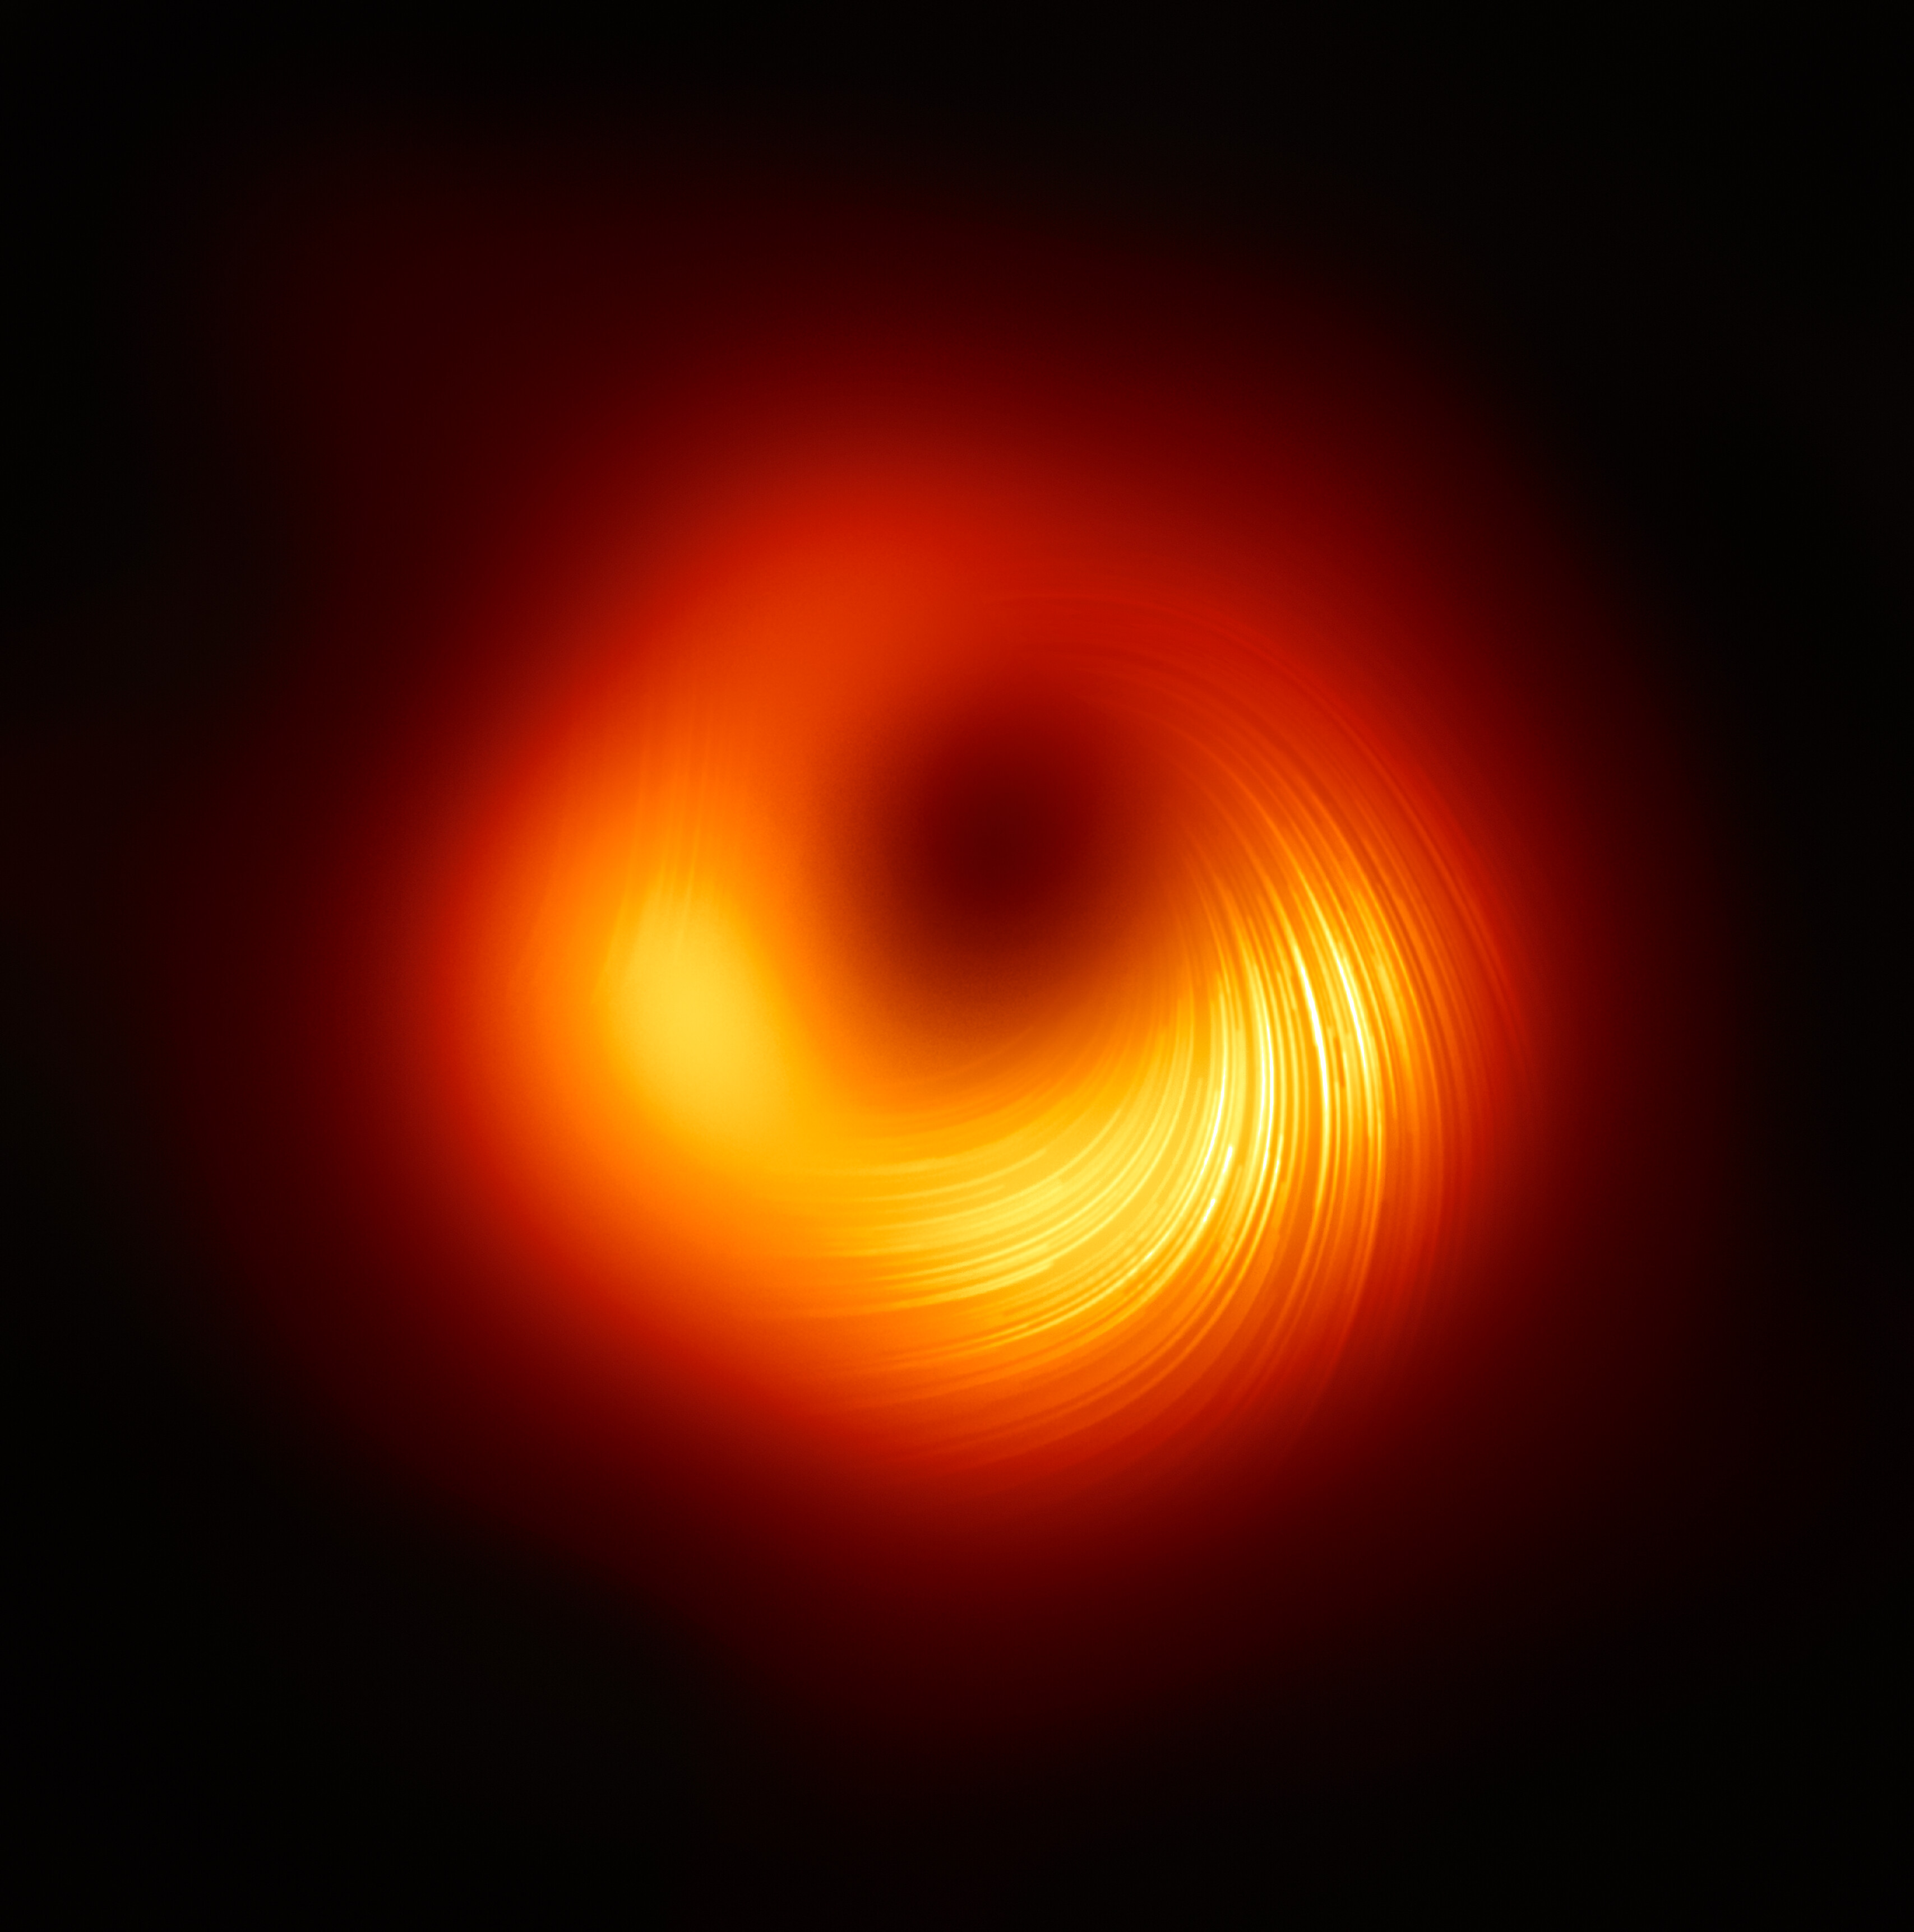
\includegraphics[width=0.7\linewidth]{
		c96e01c894dab21d52bb0bd6565f0331.jpg}
		}
	\caption{ Восстановленная фотография тени чёрной дыры.}
	\label{fig:vosstanovlennaya_fotografiya_chyornoj_dyry}
\end{figure}
			\end{lstlisting}
			}
			\end{column}%
			\hfill%
			\begin{column}{.48\textwidth}
% 				\color{blue}\rule{\linewidth}{4pt}
				\begin{figure}[H]
					\center{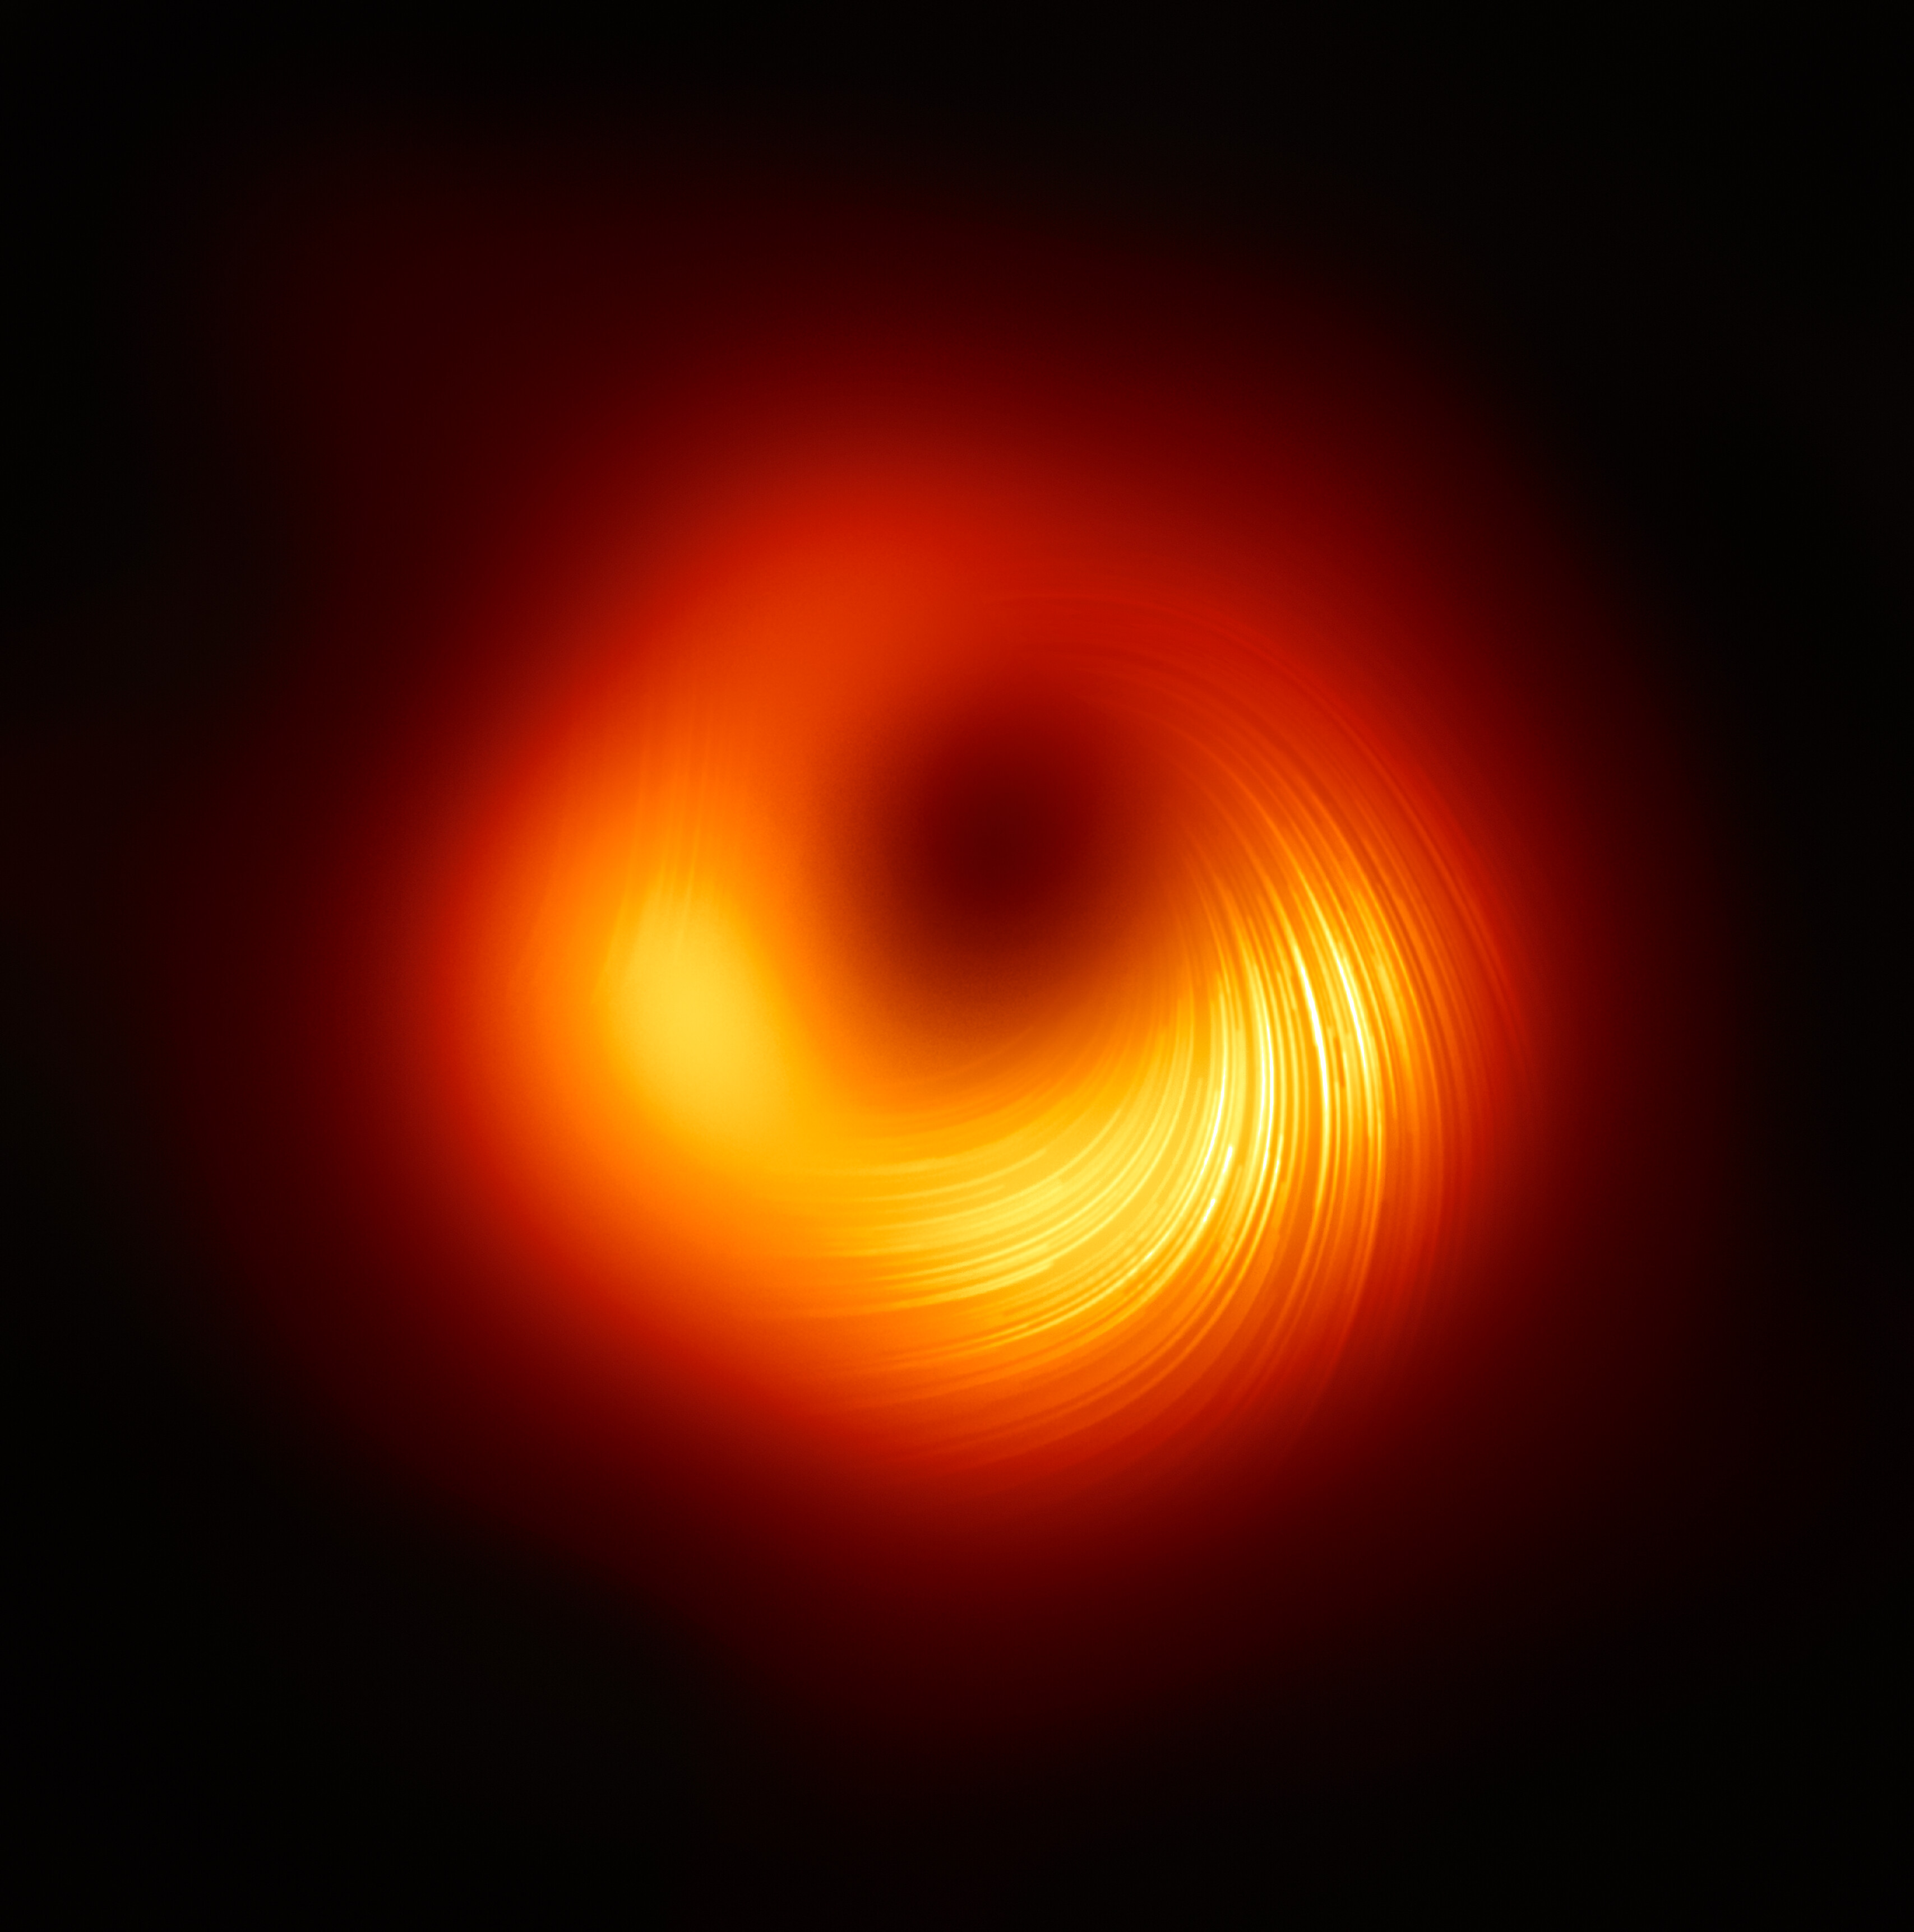
\includegraphics[width=0.7\linewidth]{c96e01c894dab21d52bb0bd6565f0331.jpg}}
					\caption{Восстановленная фотография тени чёрной дыры.}
					\label{fig:vosstanovlennaya_fotografiya_chyornoj_dyry}
				\end{figure}
			\end{column}%
		\end{columns}
		Заметим параметр <<[H]>> окружения \textsc{figure}. Этот параметр определяет место рисунка в тексте: разрешить алгоритмам ТеХа принять решение исходя из заполненности страницы.
	}
\end{frame}

\begin{frame}[squeeze, fragile]
   \label{frame:rabota_s_grafikoj}
  \frametitle{Работа с графикой}
%    \vspace{\headheight}
%    \vspace*{-5.5ex plus 1fill}
%    {\centering\bfseries%
%       \large\underline{Ввод формул и их нумерация} \\
%    }
%    \medskip
	{%\footnotesize
		Данный параметр у окружения \textsc{figure} может принимать следующие значения:
		\begin{itemize}
			\item {[h]} "--- "хотелось бы картинку здесь";
			\item настойчиво просить разместить после текста [h!] "--- "очень хочу картинку здесь";
			\item и ударить кулаком по столу "--- картинку тут и точка [H] "--- "ХОЧУ картинку здесь и баста";
			\item а с прибавлением буквы "p" мы заставляем поместить ЛаТеХ картинку отдельно на страницу так [pH] "---~см.~\url{https://mydebianblog.blogspot.com/2008/12/latex_15.html}.
		\end{itemize}
	}
\end{frame}

\begin{frame}[squeeze, fragile]
   \label{frame:rabota_s_gnuplot}
  \frametitle{Работа с \texttt{Gnuplot}}
%    \vspace{\headheight}
%    \vspace*{-5.5ex plus 1fill}
%    {\centering\bfseries%
%       \large\underline{Ввод формул и их нумерация} \\
%    }
%    \medskip
	{\footnotesize
		Теперь попытаемся построить рисунок (графики) с помощью \texttt{gnuplot} и одноимённого с ним окружения из пакета \textsc{gnuplottex}.
% 		\lstset{language = Gnuplot, frame = none, tabsize = 3, numbers = left, numbersep = 6pt, gobble=1}%
		\vbox{\vspace*{-3ex}
			\hspace*{8mm}\hbox to \paperwidth{%
				\begin{lstlisting}[language = Gnuplot, frame = none, tabsize = 3, numbers = left, numbersep = 6pt, gobble=1]
\begin{figure}[h]%
	\centering%
	\begin{gnuplot}[terminal = epslatex, terminaloptions = {color dashed size 3.0in,2.25in font ',8'}]
		set key box top left
		set key width 4
		set sample 1000
		set xr [-5:5]
		set yr [-1:1]
		set xlabel '$x$-label'
		set ylabel '$y$-label'
		plot sin(x) w l lc 1 t '$\sin(x)$',\
		cos(x) w l lc 2 t '$\cos(x)$',\
		tan(x) w l lc 3 t '$\tan(x)$',\
		tanh(x) w l lc 4 t '$5\tanh(x)$'
	\end{gnuplot}
	\caption{This is a simple example using the latex-terminal.}%
	\label{fig:latex}%
\end{figure}
				\end{lstlisting}
			}
		}
	}
\end{frame}

\begin{frame}[squeeze, fragile]
   \label{frame:primer_grafika_v_gnuplot}
  \frametitle{Пример графика в \texttt{Gnuplot}}
%    \vspace{\headheight}
%    \vspace*{-5.5ex plus 1fill}
%    {\centering\bfseries%
%       \large\underline{Ввод формул и их нумерация} \\
%    }
%    \medskip
	{\footnotesize
		%\begin{gnuplot}[terminal=pdf,terminaloptions=font ”,10” linewidth 3]
		\begin{figure}[h]%
			\centering%
			\begin{gnuplot}[terminal = epslatex, terminaloptions = {color dashed size 3.0in,2.25in font ',8'}]
				set key box top left
				set key width 4
				set sample 1000
				set xr [-5:5]
				set yr [-1:1]
				set xlabel '$x$-label'
				set ylabel '$y$-label'
				plot sin(x) w l lc 1 t '$\sin(x)$',\
				cos(x) w l lc 2 t '$\cos(x)$',\
				tan(x) w l lc 3 t '$\tan(x)$',\
				tanh(x) w l lc 4 t '$5\tanh(x)$'
			\end{gnuplot}
			\caption{Пример работы \texttt{gnuplot}.}%
			\label{fig:primer_raboty_gnuplot}%
		\end{figure}%
	}
\end{frame}

\begin{frame}[squeeze, fragile]
   \label{frame:primer_programmy_na_yazyke_fortran}
  \frametitle{Пример программы на языке \texttt{Fortran}}
%    \vspace{\headheight}
%    \vspace*{-5.5ex plus 1fill}
%    {\centering\bfseries%
%       \large\underline{Ввод формул и их нумерация} \\
%    }
%    \medskip
	{\footnotesize
		Расмотрим пример построения блок-схем с использованием пакета \textsc{tikz} с подключёнными библиотеками \textsl{arrows} и \textsl{shapes} перечислив их в \{~\}\nobreak-скобках команды \textsc{usetikzlibrary}, для построения графов же "--- \textsl{graphs}. Описание блок схем помещаются в тело окружения \textsc{tikzpicture}: узлы вводятся и описываюся командой \textsc{node}, а пути - командой \textsc{path}. Пусть нам нужно описать алгоритм программы \texttt{testx3p}, написаной на фортране (см.~директорию~\textsl{app}):

		%\VerbatimInput[frame = none, label = {Листинг программы \texttt{testx3p}}, fontfamily = courier, tabsize = 3, numbers = left, numbersep = 6pt]{src/testx3p.f08}%
		\hspace*{8mm}\hbox to \paperwidth{%
			\lstset{language = [08]Fortran, frame = none, name = {Листинг программы \texttt{testx3p}}, tabsize = 3, numbers = left, numbersep = 6pt}\lstinputlisting{src/testx3p.f08}%
		}
	}
\end{frame}

\begin{frame}[squeeze, fragile]
   \label{frame:rabota_s_blok_sxemami}
  \frametitle{Работа с блок\nobreak-схемами}
%    \vspace{\headheight}
%    \vspace*{-5.5ex plus 1fill}
%    {\centering\bfseries%
%       \large\underline{Ввод формул и их нумерация} \\
%    }
%    \medskip
	{\footnotesize
		Для удобства опишем несколько \textsl{tikz}\nobreak-стилей согласно \textbf{ГОСТ 19.701-90 <<Схемы алгоритмов программ, данных и систем>>} "---~см.~\cite{mkrtumyan:tech:2010:01}, с помощью команды \textsc{tikzset}:

		\Verb|\tikzset{<имя_стиля>/.style = {<параметры_стиля>}}|.

		Используемые стили см.~в исходном tex\nobreak-файле настоящей\\ статьи. Таким образом,

		{
% 		\begin{columns}[T] % align columns
% 			\begin{column}{.48\textwidth}
% 				\color{red}\rule{\linewidth}{4pt}
% 			\end{column}%
% 			\hfill%
% 			\begin{column}{.48\textwidth}
% 				\color{blue}\rule{\linewidth}{4pt}
% 			\end{column}%
% 		\end{columns}
		\begin{columns}[T] % align columns
			\begin{column}{.48\textwidth}
% 			\color{red}\rule{\linewidth}{4pt}
				\begin{tikzpicture}[node distance = 1.0cm, auto]
					\node [terminator] at (0,0) (start) {\textbf{Начало}};
					\node [data, below of = start, node distance=1.0cm] (input) {$x$, $y$, $i$, $j$, $n$, массив $p$};
					\node [operator, below of = input, node distance=1.0cm] (openfile) {Открыть файл \textsl{data.res}, id = n};
					\node [operator, below of = openfile, node distance=1.0cm] (output1) {Записать {\tt $p[~]$} в файл \textsl{data.res}};
					\node [connector, below of = output1, node distance=1.0cm] (connectorin1) {1};
					\path [draw, -latex'] (start) edge (input);
					\path [-] (input) edge (openfile);
					\path [-] (openfile) edge (output1);
					\path [-] (output1) edge (connectorin1);
				\end{tikzpicture}
			\end{column}%
			\hfill%
			\begin{column}{.48\textwidth}
% 				\color{blue}\rule{\linewidth}{4pt}
				\vspace*{-5ex}
% 				\hspace*{-7ex}
				\begin{tikzpicture}[node distance = 1.0cm, auto]
					\node [connector] at (0,0) (connectorout1) {1};
					\node [loop, below of = connectorout1, node distance=1.0cm, draw, text width=3cm] (loop) {Главный цикл расчёта \\ $i = \overline{0,20}$};
					\node [operator, below of = loop, node distance=1.0cm] (calculation) {$x = -1 + i 0,1$};
					\node [operator, below of = calculation, node distance=1.0cm, draw, text width=4cm] (output2) {Записать {\tt $x$, $(x + p_{j})^{3}$ $\forall j = \overline{-4,4}$} \\ в файл \textsl{data.res}};
					\node [endloop, below of = output2, node distance=1.0cm] (endloop) {Главный цикл расчёта};
					\node [terminator, below of = endloop, node distance=1.0cm] (end) {\textbf{Конец}};
					\path [-] (connectorout1) edge (loop);
					\path [-] (loop) edge (calculation);
					\path [-] (calculation) edge (output2);
					\path [-] (output2) edge (endloop);
					\path [-] (endloop) edge (end);
				\end{tikzpicture}
			\end{column}%
			\end{columns}

		}
	}
\end{frame}

\begin{frame}[squeeze, fragile]
   \label{frame:primer_stilya_blok_sxemy}
  \frametitle{Пример стиля блок\nobreak-схемы}
%    \vspace{\headheight}
%    \vspace*{-5.5ex plus 1fill}
%    {\centering\bfseries%
%       \large\underline{Ввод формул и их нумерация} \\
%    }
%    \medskip
	{\footnotesize
		Для случая блок\nobreak-схемы вызова внешней подпрограммы (см.~\url{https://pro-prof.com/archives/1462}) мы используем следующий стиль:
		\hspace*{8mm}\hbox to \paperwidth{%
			\begin{lstlisting}[frame = none, linewidth = 0.85\paperwidth, basicstyle=\tiny, caption = {Пример стиля \textsc{tikz}}, label = {primer_stilya_tikz}]
\tikzset{subroutine/.style = {% блок вызова внешней подпрограммы
		rectangle split, rectangle split horizontal,
		rectangle split parts = 3,
		draw, text centered,
		minimum width = 5em,
		minimum height = 2em,
		outer sep = 0
	}
}%
\begin{tikzpicture}
	\node [subroutine] at (0,0) (subroutine) {\nodepart{two}\textbf{Подпрограмма}};
\end{tikzpicture}\%
			\end{lstlisting}
		}
{
		\begin{tikzpicture}
			\node [subroutine] at (0,0) (subroutine) {\nodepart{two}\textbf{Подпрограмма}};
		\end{tikzpicture}
}\\
		Обратите внимание, что для корректной работы перед содержимым блока в \textsc{node} необходимо прописать \lstinline|\nodepart{two}|.

		Описание tikz\nobreak-стилей (да и других) рекомендуется сохранять в отдельном tex\nobreak-файле и подключать его в преамбуле, или в начале тело документа с помощью команды \textsc{input}.
%
}
\end{frame}

\begin{frame}[squeeze, fragile, allowframebreaks]
   \label{frame:grafiki_rezultata_raboty_programmy_testx3p}
  \frametitle{Графики результата работы программы \texttt{testx3p}}
%    \vspace{\headheight}
%    \vspace*{-5.5ex plus 1fill}
%    {\centering\bfseries%
%       \large\underline{Ввод формул и их нумерация} \\
%    }
%    \medskip
	{%\footnotesize
% 		\begin{columns}[T] % align columns
% 			\begin{column}{.48\textwidth}
		Построим график из данных расчёта программы \texttt{testx3p}.


		Результаты расчёта записываются программой в файл \textsl{testx3p.res} в поддиректорию \textsl{data}. После небольшой обработки содержимомго файла под нужды пакета \textsc{tabularray} и записи результата в файл \textsl{tbl1.tex} в поддиректорию \textsl{tables} мы можем представить эти данные в табличной виде~(см.~табл. 2).

	Путь к исходному файлу с данными \textsl{testx3p.res} мы пропишем в сам скрипт gnuplot для построения графиков, который сохраним в отдельном файле, а затем подключим его в \TeX\ документ с помощью команды \textsc{gnuplotloadfile}, например \\ \Verb|\gnuplotloadfile[<параметры>]{scr/testx3p1.gp}|. Подробнее этот пример программы на \textsl{фортране} и взаимодействия с \texttt{gnuplot} см.~\cite{shnejvajs:book:2016:01}.
% 	\end{column}
% 	\begin{column}{.50\textwidth}
	\begin{figure}[pH]%
		\centering%
		\gnuplotloadfile[terminal = epslatex, terminaloptions = {color dashed size 6.0in,3.25in font ',8'}]{scr/testx3p1.gp}
% 		\gnuplotloadfile[terminal = epslatex, terminaloptions = {color dashed size 3.0in,2.25in font ',5'}]{scr/testx3p1.gp}
		\caption{Семейство кривых функции $f(x) = (x + p)^{3}$.}%
		\label{fig:semejstvo_krivyx_funkcii_fx}%
	\end{figure}%
% 	\end{column}
% 	\end{columns}
}
\end{frame}

\begin{frame}[squeeze, fragile]%, allowframebreaks]
   \label{frame:listing_gnuplot_skripta_dlya_grafikov_programmy_testx3p}
  \frametitle{\texttt{Gnuplot}\nobreak-скрипт для графиков программы \texttt{testx3p}}
	{\fontsize{4.3pt}{4.4}\selectfont
		\vbox{\vspace*{-3ex}
			\hspace*{8mm}\hbox to \paperwidth{%
				\lstinputlisting[language = Gnuplot, frame = none, tabsize = 3, numbers = left, numbersep = 6pt, gobble=1]{scr/testx3p1.gp}
			}
		}

	}
\end{frame}

%
%

\begin{frame}[squeeze, fragile]%, allowframebreaks]
   \label{frame:tablica_rezultatov_raboty_programmy_testx3p}
  \frametitle{Таблица результатов работы программы \texttt{testx3p}}
	{\fontsize{4.3pt}{4.4}\selectfont
		%{{{ Horrible hack

		\ExplSyntaxOn
		% read the file content
		\file_get:nnN {tables/tbl1} {\ExplSyntaxOff} \tblone
		\ExplSyntaxOff

		%}}}

% 		\vspace*{-3ex}
		\begin{longtblr}[
		% 	theme = fancy,
			caption = {Результаты расчёта программы \texttt{testx3p}.},
			entry = {Расчёта программы \texttt{testx3p}.},
			label = {tblr:rezultaty_raschyota_programmy_testx3p},
		% 	note{a} = {Это первая сноска.},
		% 	note{$\dag$} = {Это вторая длинная сноска.},
		% 	remark{Примечание} = {Некоторые общие примечания.},
		% 	remark{Источник} = {Сделано силами авторов.},
			baseline = m,
			expand = \expandafter,
		]{
			rows = {c},
			columns = {r},
			row{odd} = {bg = red8},
			row{1} = {m,bg = red3, fg = white, font = \sffamily},
% 			row{1}{1} = {c},
			rowhead = 1,
			rowfoot = 0,
			width=\textwidth,
			hlines,
			vlines,
		}
			%	\diagbox{x}{p} & -0,90 & -0,50 & -0,30 & -0,10 & 0,00 & 0,10 & 0,30 & 0,50 & 0,90 \\
	-1,00 & -6,86 & -3,38 & -2,20 & -1,33 & -1,00 & -0,73 & -0,34 & -0,12 & -0,00 \\
	-0,90 & -5,83 & -2,74 & -1,73 & -1,00 & -0,73 & -0,51 & -0,22 & -0,06 & 0,00 \\
	-0,80 & -4,91 & -2,20 & -1,33 & -0,73 & -0,51 & -0,34 & -0,12 & -0,03 & 0,00 \\
	-0,70 & -4,10 & -1,73 & -1,00 & -0,51 & -0,34 & -0,22 & -0,06 & -0,01 & 0,01 \\
	-0,60 & -3,38 & -1,33 & -0,73 & -0,34 & -0,22 & -0,12 & -0,03 & -0,00 & 0,03 \\
	-0,50 & -2,74 & -1,00 & -0,51 & -0,22 & -0,12 & -0,06 & -0,01 & 0,00 & 0,06 \\
	-0,40 & -2,20 & -0,73 & -0,34 & -0,12 & -0,06 & -0,03 & -0,00 & 0,00 & 0,12 \\
	-0,30 & -1,73 & -0,51 & -0,22 & -0,06 & -0,03 & -0,01 & 0,00 & 0,01 & 0,22 \\
	-0,20 & -1,33 & -0,34 & -0,12 & -0,03 & -0,01 & -0,00 & 0,00 & 0,03 & 0,34 \\
	-0,10 & -1,00 & -0,22 & -0,06 & -0,01 & -0,00 & 0,00 & 0,01 & 0,06 & 0,51 \\
	0,00 & -0,73 & -0,12 & -0,03 & -0,00 & 0,00 & 0,00 & 0,03 & 0,12 & 0,73 \\
	0,10 & -0,51 & -0,06 & -0,01 & 0,00 & 0,00 & 0,01 & 0,06 & 0,22 & 1,00 \\
	0,20 & -0,34 & -0,03 & -0,00 & 0,00 & 0,01 & 0,03 & 0,13 & 0,34 & 1,33 \\
	0,30 & -0,22 & -0,01 & 0,00 & 0,01 & 0,03 & 0,06 & 0,22 & 0,51 & 1,73 \\
	0,40 & -0,12 & -0,00 & 0,00 & 0,03 & 0,06 & 0,12 & 0,34 & 0,73 & 2,20 \\
	0,50 & -0,06 & 0,00 & 0,01 & 0,06 & 0,12 & 0,22 & 0,51 & 1,00 & 2,74 \\
	0,60 & -0,03 & 0,00 & 0,03 & 0,12 & 0,22 & 0,34 & 0,73 & 1,33 & 3,38 \\
	0,70 & -0,01 & 0,01 & 0,06 & 0,22 & 0,34 & 0,51 & 1,00 & 1,73 & 4,10 \\
	0,80 & -0,00 & 0,03 & 0,13 & 0,34 & 0,51 & 0,73 & 1,33 & 2,20 & 4,91 \\
	0,90 & 0,00 & 0,06 & 0,22 & 0,51 & 0,73 & 1,00 & 1,73 & 2,74 & 5,83 \\
	1,00 & 0,00 & 0,12 & 0,34 & 0,73 & 1,00 & 1,33 & 2,20 & 3,38 & 6,86 \\
 % не работает!
			\expandafter\empty\tblone

		\end{longtblr}
}
\end{frame}

%
%

%заключение
\section{Заключение}
\label{sec:zaklyuchenije}

\begin{frame}[squeeze, fragile]
   \label{frame:zaklyuchenije}
  \frametitle{Заключение}
%    \vspace{\headheight}
%    \vspace*{-5.5ex plus 1fill}
%    {\centering\bfseries%
%       \large\underline{Ввод формул и их нумерация} \\
%    }
%    \medskip
	{\footnotesize
		В заключении отметим, что данное руководство в большей степени пример; для полнового введения лучше обратиться к справичникам и к указанной литературе. По-началу поттребуется много практики для освоения языка программирования \LaTeX. Вместе с тем \texttt{gnuplot} был выбран из-за простоти в его освоении, и хорошей связки с \LaTeX. Тем не менее, можно строить графики средствами самого \LaTeX а, а именно при помощи того же пакета \textsc{tikz}, использованного для построения блок-схем. Однако рекомендуется сначала освоиться с \textsl{базовым} \LaTeX ом.
	}
\end{frame}


% \section*{\refname}
% \addtocontents{toc}{section}{Список литературы}
\label{sec:literatura}


\begin{frame}[t, squeeze, fragile, allowframebreaks]
   \label{frame:literatura}
  \frametitle{Список литературы}
%    \vspace{\headheight}
%    \vspace*{-5.5ex plus 1fill}
%    {\centering\bfseries%
%       \large\underline{Ввод формул и их нумерация} \\
%    }
%    \medskip
	{\footnotesize
		% \bibliographystyle{gost7184}
		\bibliography{bib/main}
	}
\end{frame}

% \newpage
% \section{Приложение}
% \label{sec:prilozhenije}


%{{{ Horrible hack

%\ExplSyntaxOn
%% read the file content
%\file_get:nnN {tables/tbl2} {\ExplSyntaxOff} \tbltwo
%\ExplSyntaxOff

%}}}

% \begin{frame}[squeeze, fragile, allowframebreaks]
%    \label{frame:prilozhenije}
%   \frametitle{Приложение}
% 	{\footnotesize
% 		\begin{longtblr}[
% 		% 	theme = fancy,
% 			caption = {Результаты моделирования движения частицы.},
% 			entry = {Баллистическое движение частицы.},
% 			label = {tblr:rezultaty_modelirovaniya_dvizheniya_chasticy},
% 		% 	note{a} = {Это первая сноска.},
% 		% 	note{$\dag$} = {Это вторая длинная сноска.},
% 		% 	remark{Примечание} = {Некоторые общие примечания.},
% 		% 	remark{Источник} = {Сделано силами авторов.},
% 			baseline = m,
% 			expand=\expandafter,
% 		]{
% 			rows = {c},
% 			columns = {r},
% 			row{odd} = {bg = azure8},
% 			row{1-2} = {c, bg = azure3, fg = white, font = \sffamily},
% 			rowhead = 2,
% 			rowfoot = 0,
% 			width=\textwidth,
% 			hlines,
% 			vlines,
% 		}
% 		% 	\hline
% 				\SetCell[r = 2]{c} {Время \\ $t$, с}
% 					& \SetCell[c = 2]{c} {Координаты}
% 						&	& \SetCell[c = 2]{c} {Скорость} & \\
% 		% 	\hline
% 					& $x$, м & $y$, м & $v_{x}$, м/с & $v_{y}$, м/с \\
% 		% 	\hline
% 			%	\diagbox{x}{p} & -0,90 & -0,50 & -0,30 & -0,10 & 0,00 & 0,10 & 0,30 & 0,50 & 0,90 \\
	-1,00 & -6,86 & -3,38 & -2,20 & -1,33 & -1,00 & -0,73 & -0,34 & -0,12 & -0,00 \\
	-0,90 & -5,83 & -2,74 & -1,73 & -1,00 & -0,73 & -0,51 & -0,22 & -0,06 & 0,00 \\
	-0,80 & -4,91 & -2,20 & -1,33 & -0,73 & -0,51 & -0,34 & -0,12 & -0,03 & 0,00 \\
	-0,70 & -4,10 & -1,73 & -1,00 & -0,51 & -0,34 & -0,22 & -0,06 & -0,01 & 0,01 \\
	-0,60 & -3,38 & -1,33 & -0,73 & -0,34 & -0,22 & -0,12 & -0,03 & -0,00 & 0,03 \\
	-0,50 & -2,74 & -1,00 & -0,51 & -0,22 & -0,12 & -0,06 & -0,01 & 0,00 & 0,06 \\
	-0,40 & -2,20 & -0,73 & -0,34 & -0,12 & -0,06 & -0,03 & -0,00 & 0,00 & 0,12 \\
	-0,30 & -1,73 & -0,51 & -0,22 & -0,06 & -0,03 & -0,01 & 0,00 & 0,01 & 0,22 \\
	-0,20 & -1,33 & -0,34 & -0,12 & -0,03 & -0,01 & -0,00 & 0,00 & 0,03 & 0,34 \\
	-0,10 & -1,00 & -0,22 & -0,06 & -0,01 & -0,00 & 0,00 & 0,01 & 0,06 & 0,51 \\
	0,00 & -0,73 & -0,12 & -0,03 & -0,00 & 0,00 & 0,00 & 0,03 & 0,12 & 0,73 \\
	0,10 & -0,51 & -0,06 & -0,01 & 0,00 & 0,00 & 0,01 & 0,06 & 0,22 & 1,00 \\
	0,20 & -0,34 & -0,03 & -0,00 & 0,00 & 0,01 & 0,03 & 0,13 & 0,34 & 1,33 \\
	0,30 & -0,22 & -0,01 & 0,00 & 0,01 & 0,03 & 0,06 & 0,22 & 0,51 & 1,73 \\
	0,40 & -0,12 & -0,00 & 0,00 & 0,03 & 0,06 & 0,12 & 0,34 & 0,73 & 2,20 \\
	0,50 & -0,06 & 0,00 & 0,01 & 0,06 & 0,12 & 0,22 & 0,51 & 1,00 & 2,74 \\
	0,60 & -0,03 & 0,00 & 0,03 & 0,12 & 0,22 & 0,34 & 0,73 & 1,33 & 3,38 \\
	0,70 & -0,01 & 0,01 & 0,06 & 0,22 & 0,34 & 0,51 & 1,00 & 1,73 & 4,10 \\
	0,80 & -0,00 & 0,03 & 0,13 & 0,34 & 0,51 & 0,73 & 1,33 & 2,20 & 4,91 \\
	0,90 & 0,00 & 0,06 & 0,22 & 0,51 & 0,73 & 1,00 & 1,73 & 2,74 & 5,83 \\
	1,00 & 0,00 & 0,12 & 0,34 & 0,73 & 1,00 & 1,33 & 2,20 & 3,38 & 6,86 \\
 % не работает!
% 			\expandafter\empty\tbltwo
% 		\end{longtblr}
% 	}
% \end{frame}


\end{document}
